\documentclass[tikz,border=2pt,11pt]{standalone}
\usepackage{xfp}
\usetikzlibrary{arrows.meta,calc}

% Illustrative parameters in keV and energies derived from the alpha Q values.
\providecommand{\RfBEx}{110}
\providecommand{\HsDelta}{20}
\def\DsEx{300}
\edef\SgAEx{\fpeval{152.299-\RfBEx}}
\edef\HsLowEx{\fpeval{30.418+\RfBEx}}
\edef\HsRotEx{\fpeval{\HsLowEx+\HsDelta}}
\edef\HsHighEx{\fpeval{\RfBEx-22.962+\HsDelta}}

\definecolor{alphared}{RGB}{179,65,47}
\definecolor{itblue}{RGB}{47,92,143}
\definecolor{sfgreen}{RGB}{56,120,91}
\pgfdeclarelayer{transitions}
\pgfsetlayers{transitions,main}

\def\levelwidth{1.92} % cm
\edef\itx{\fpeval{\levelwidth-0.14}} % cm from the left end of each level

\newcommand{\drawnuclide}[3]{%
  % Each entry is state ID / excitation energy / orbital label / line style.
  \foreach \stateid/\energy/\orbital/\linestyle in {#3} {
    \coordinate (\stateid-L) at (#1,\energy);
    \coordinate (\stateid-R) at ({#1+\levelwidth},\energy);
    \draw[level,\linestyle] (\stateid-L) -- (\stateid-R);
    \node[orbital label,at={(\stateid-L)},\stateid\space orbital/.try] {$\orbital$};
  }
  \node[nuclide label] at ({#1+\levelwidth/2},-13) {$#2$};
}

\begin{document}
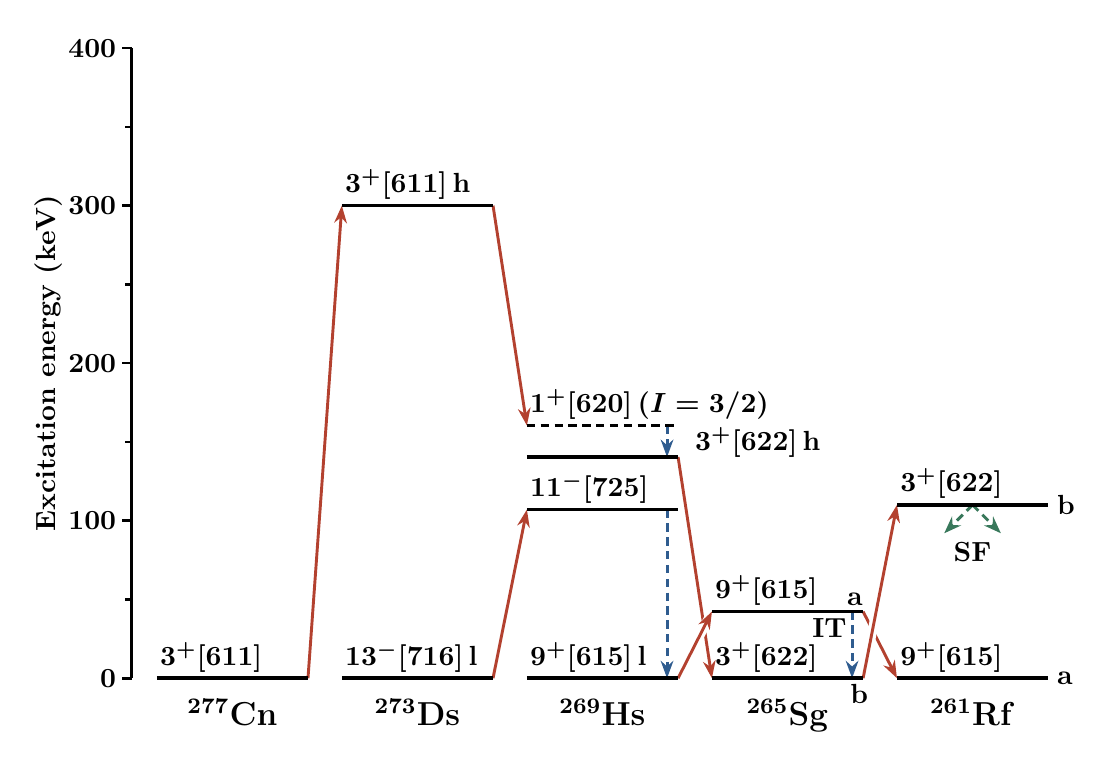
\begin{tikzpicture}[x=1cm,y=0.02cm,every node/.style={font=\bfseries\boldmath}]
  % Parkhomenko geometry, extended by two columns.
  \path[use as bounding box] (-0.29,-37) rectangle (13.12,413);
  \tikzset{
    level/.style={black,line width=1.3pt},
    axis/.style={black,line width=0.95pt},
    orbital label/.style={
      anchor=south west,xshift=1pt,yshift=2pt,inner sep=0pt
    },
    hs-low orbital/.style={at={(hs-low-R)},xshift=5pt,yshift=-2.5pt},
    nuclide label/.style={anchor=north,inner sep=0pt,font=\large\bfseries\boldmath},
    level index/.style={anchor=west,xshift=3pt,inner sep=0pt},
    decay/.style={-{Stealth[length=2.2mm,width=1.6mm]},line width=1.05pt},
    alpha decay/.style={decay,alphared},
    it decay/.style={decay,itblue,densely dashed},
    sf decay/.style={decay,sfgreen,densely dashed},
    crossing/.style={preaction={draw=white,line width=3.4pt,-}},
    mode label/.style={inner sep=1.5pt,text=black}
  }

  \draw[axis] (1.03,0) -- (1.03,400);
  \foreach \energy in {0,100,200,300,400} {
    \draw[axis] (0.91,\energy) -- (1.03,\energy);
    \node[anchor=east,inner sep=0pt]
      at (0.84,\energy) {\energy};
  }
  \foreach \energy in {50,150,250,350} {
    \draw[axis] (0.95,\energy) -- (1.03,\energy);
  }
  \node[rotate=90,inner sep=0pt]
    at (-0.03,200) {Excitation energy (keV)};

  % Compact 2 Omega labels for single-particle states. The dashed [620]
  % level is the I=3/2 rotational member built on the 1/2+ orbital.
  \drawnuclide{1.35}{^{277}\mathrm{Cn}}{
    cn-g/0/{3^{+}[611]}/solid%
  }
  \drawnuclide{3.70}{^{273}\mathrm{Ds}}{
    ds-g/0/{13^{-}[716]\,\mathrm{l}}/solid,
    ds-ex/\DsEx/{3^{+}[611]\,\mathrm{h}}/solid%
  }
  \drawnuclide{6.05}{^{269}\mathrm{Hs}}{
    hs-g/0/{9^{+}[615]\,\mathrm{l}}/solid,
    hs-high/\HsHighEx/{11^{-}[725]}/solid,
    hs-low/\HsLowEx/{3^{+}[622]\,\mathrm{h}}/solid,
    hs-rot/\HsRotEx/{1^{+}[620]\,(I=3/2)}/densely dashed%
  }
  \drawnuclide{8.40}{^{265}\mathrm{Sg}}{
    sg-b/0/{3^{+}[622]}/solid,
    sg-a/\SgAEx/{9^{+}[615]}/solid%
  }
  \drawnuclide{10.75}{^{261}\mathrm{Rf}}{
    rf-a/0/{9^{+}[615]}/solid,
    rf-b/\RfBEx/{3^{+}[622]}/solid%
  }
  \node[orbital label,anchor=south east,xshift=-1pt] at (sg-a-R) {a};
  \node[level index,anchor=north east,xshift=-1pt,yshift=-2pt] at (sg-b-R) {b};
  \node[level index] at (rf-a-R) {a};
  \node[level index] at (rf-b-R) {b};

  \begin{pgfonlayer}{transitions}
    \draw[alpha decay] (cn-g-R) -- (ds-ex-L);
    \draw[alpha decay] (ds-ex-R) -- (hs-rot-L);
    \draw[alpha decay] (ds-g-R) -- (hs-high-L);
    \draw[alpha decay] (hs-low-R) -- (sg-b-L);
    \draw[alpha decay,crossing] (hs-g-R) -- (sg-a-L);
    \draw[alpha decay] (sg-a-R) -- (rf-a-L);
    \draw[alpha decay,crossing] (sg-b-R) -- (rf-b-L);

    \draw[it decay] ($(hs-rot-L)+(\itx,0)$)
      -- node[mode label,right] {} ($(hs-low-L)+(\itx,0)$);
    \draw[it decay] ($(hs-high-L)+(\itx,0)$)
      -- node[mode label,left] {} ($(hs-g-L)+(\itx,0)$);
    \draw[it decay] ($(sg-a-L)+(\itx,0)$)
      -- node[mode label,left,pos=.25] {IT} ($(sg-b-L)+(\itx,0)$);

    % The x and y displacements are equal in physical units (0.36 cm).
    \coordinate (sf-apex) at ($(rf-b-L)+(\levelwidth/2,0)$);
    \draw[sf decay] (sf-apex) -- ++(-.36,-18);
    \draw[sf decay] (sf-apex) -- ++( .36,-18);
  \end{pgfonlayer}
  \node[mode label,anchor=north] at ($(sf-apex)+(0,-21)$) {SF};
\end{tikzpicture}
\end{document}
